\section{Tekniskt bidrag}% "Contributions" -- Syfte.
Med en budget på 5000 kr har ett system innehållande en robothand med tre fingrar som styrs trådlöst med en styrhandske utvecklats. Utifrån Cutkoskys grepphierarki, se Appendix~\ref{cutshand}, utformas robothanden och dess fingrar för att möjliggöra ett stort antal olika grepp, med olika krav på styrka, omfång, finkänslighet och fingerfärdighet. Grunden till den mekaniska konstruktionen utgörs av Meccano med följden att delarna blir standardiserade och behovet att tillverka mekaniska delar kringgås. Meccano är ett modellkonstruktionskit som består av återanvändbara metalldelar och plastdelar med muttrar och skruvar för att sätt ihop delarna. Totalt har robothanden åtta leder varav sex är separat styrbara och aktueras av varsin servomotor. Robothandens fingrar har ett människolikt rörelsemönster för att användaren intuitivt skall kunna styra den med sina egna fingrar via styrhandsken.

För att styrhandsken skall passa olika händer kalibreras den enkelt av användaren själv med två knapptryckningar. I styrhandsken registrerar sex flexresistorer användarens fingerrörelser. Mätvärdena från dessa behandlas av en \emph{Arduino Micro} som sedan trådlöst kommunicerar med robothandens \emph{Arduino Due} där dessa används som styrsignaler till servomotorerna.\\ För att undvika skador på objekt mäter robothanden kontakttrycket med hjälp av trycksensorer på fingertopparna, vars mätvärden återkopplas till användaren via ledramper som lyser upp proportionerligt mot uppmätt tryck. För att ytterligare förbättra hanteringen av objekt kan robothanden identifiera vissa kända objekt och sedan assistera användaren genom att begränsa kontakttrycket mellan fingertopparna och objektet. Identifieringen sker genom att robothanden mäter avståndet mellan fingertopparna då trycksensorerna kommer i kontakt med ett objekt, detta avstånd jämförs sedan mot en lista innehållande fördefinerade objekt efter detta mått, samt vilket kontaktryck sensorerna bör registrera vid hantering av objektet. Robothanden tillåter sedan inte att högre kontakttryck uppstår tills användaren släpper objektet och den återgår till normal drift.

Nedan visas ett flödesschema för att överskådligt beskriva hur robothanden principiellt fungerar vid användande.

\begin{figure}[H]
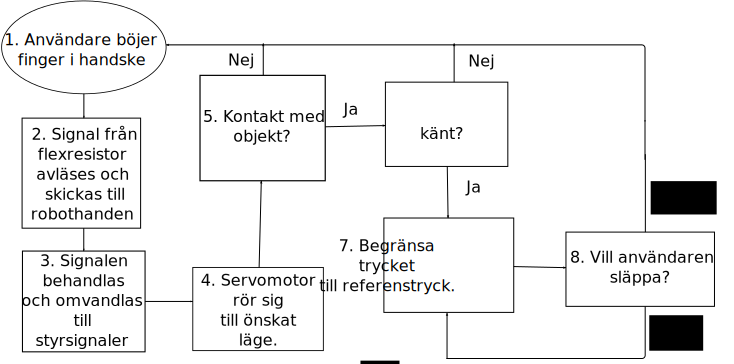
\includegraphics[width=.90\textwidth]{img/flodesschema}
\caption{Flödesschema över en tänkt signals väg genom robothanden.}
\label{flodesschema}
\end{figure}

\begin{enumerate}
\item Önskat fingerläge ges genom att användaren böjer sitt finger i kontrollhandsken.
\item Flexresistor på kontrollhandsken ändrar resistans, detta registreras i handskens \emph{Arduino Micro} som sänder detta vidare till robothandens \emph{Arduino Due} via bluetooth.
\item Signalen omvandlas till styrsignal för servomotorn.
\item Servomotorn rör sig till önskat läge för att imitera användarens fingerrörelse.
\item Trycksensorerna på fingertopparna känner av ifall något objekt greppats. Om inte (Nej), återgår systemet till att följa önskat fingerläge.
\item Om handen har gripit ett objekt försöker den identifiera det som ett av de fördefinerade, kända objekten, om detta inte lyckats (Nej) följer handen användarens önskade rörelser.
\item Om objektet identifieras som ett av de kända kommer handen inte tillåta att objektet greppas hårdare än ett fördefinerat maxtryck.
\item Tryckbegränsningen kvarstår tills användaren visar att den vill släppa objektet genom att öppna sin hand, då återgår robothanden till att följa användarens önskade rörelser igen.
\end{enumerate}




%Detta är just nu en förklaring på vårt systems funktion bara. Bör ingå mer tekniskt? Vilka medel vi använt o så.